\documentclass[xcolor=dvipsnames,table]{beamer}

\usepackage{latexsym}
\usepackage[utf8]{inputenc}
\usepackage[brazil]{babel}
\usepackage{amssymb}
\usepackage{amsmath}
\usepackage{stmaryrd}
\usepackage{fancybox}
\usepackage{datetime}
\usepackage[T1]{fontenc}
\usepackage{graphicx}
\usepackage{graphics}
\usepackage{url}
\usepackage{algorithmic}
\usepackage{algorithm}
\usepackage{acronym}
\usepackage{array}

\usepackage{listings}
\usepackage{color}

\definecolor{mygreen}{rgb}{0,0.6,0}
\definecolor{mygray}{rgb}{0.5,0.5,0.5}
\definecolor{mymauve}{rgb}{0.58,0,0.82}

\lstdefinelanguage{JavaScript}{
  keywords={typeof, new, true, false, catch, function, return, null, catch, switch, var, if, in, while, do, else, case, break},
  keywordstyle=\color{blue}\bfseries,
  ndkeywords={class, export, boolean, throw, implements, import, this},
  ndkeywordstyle=\color{darkgray}\bfseries,
  identifierstyle=\color{black},
  sensitive=false,
  comment=[l]{//},
  morecomment=[s]{/*}{*/},
  commentstyle=\color{purple}\ttfamily,
  stringstyle=\color{red}\ttfamily,
  morestring=[b]',
  morestring=[b]",
}

\lstset{ %
  backgroundcolor=\color{white},   % choose the background color; you must add \usepackage{color} or \usepackage{xcolor}
  basicstyle=\small,        % the size of the fonts that are used for the code
  breakatwhitespace=false,         % sets if automatic breaks should only happen at whitespace
  breaklines=true,                 % sets automatic line breaking
  captionpos=b,                    % sets the caption-position to bottom
  commentstyle=\color{mygreen},    % comment style
  deletekeywords={...},            % if you want to delete keywords from the given language
  escapeinside={\%*}{*)},          % if you want to add LaTeX within your code
  extendedchars=true,              % lets you use non-ASCII characters; for 8-bits encodings only, does not work with UTF-8
  frame=single,	                   % adds a frame around the code
  keepspaces=true,                 % keeps spaces in text, useful for keeping indentation of code (possibly needs columns=flexible)
  keywordstyle=\color{blue},       % keyword style
  language=HTML,                 % the language of the code
  otherkeywords={*,...},           % if you want to add more keywords to the set
  numbers=left,                    % where to put the line-numbers; possible values are (none, left, right)
  numbersep=5pt,                   % how far the line-numbers are from the code
  numberstyle=\tiny\color{mygray}, % the style that is used for the line-numbers
  rulecolor=\color{black},         % if not set, the frame-color may be changed on line-breaks within not-black text (e.g. comments (green here))
  showspaces=false,                % show spaces everywhere adding particular underscores; it overrides 'showstringspaces'
  showstringspaces=false,          % underline spaces within strings only
  showtabs=false,                  % show tabs within strings adding particular underscores
  stepnumber=1,                    % the step between two line-numbers. If it's 1, each line will be numbered
  stringstyle=\color{mymauve},     % string literal style
  tabsize=2,	                   % sets default tabsize to 2 spaces
  title=\lstname,                   % show the filename of files included with \lstinputlisting; also try caption instead of title
  moredelim=**[is][\color{purple}]{@}{@},
}

\newtheorem{definicao}{Definio}
\newcommand{\tab}{\hspace*{2em}}

\mode<presentation>
{
  \definecolor{colortexto}{RGB}{0,0,0}
 
  \setbeamertemplate{background canvas}[vertical shading][ bottom=white!10,top=white!10]
  \setbeamercolor{normal text}{fg=colortexto} 

  \usetheme{Warsaw}
}

\title{Movimento Retilíneo} 

\author{
  Esdras Lins Bispo Jr. \\ \url{bispojr@ufg.br}
  } 
 \institute{
  Física para Ciência da Computação \\Bacharelado em Ciência da Computação}
\date{\textbf{04 de setembro de 2019} }

\logo{
\includegraphics[width=1cm]{images/ufgJataiLogo.png}}

\begin{document}

	\begin{frame}
		\titlepage
	\end{frame}

	\AtBeginSection{
		\begin{frame}{Sumário}%[allowframebreaks]{Sumário}
    		\tableofcontents[currentsection]
    		%\tableofcontents[currentsection, hideothersubsections]
		\end{frame}
	}

	\begin{frame}{Plano de Aula}
		\tableofcontents
		%\tableofcontents[hideallsubsections]
	\end{frame}

%------------------------------------------
\section{Pensamento}
	\begin{frame}{Pensamento}
  		\begin{center}
    		
\includegraphics[width=7cm]{images/pensamento.png}
  		\end{center}
	\end{frame}
	
	\begin{frame}{Pensamento}
		\begin{columns}
			\column{.4\textwidth}  		
		  		\begin{center}
		    		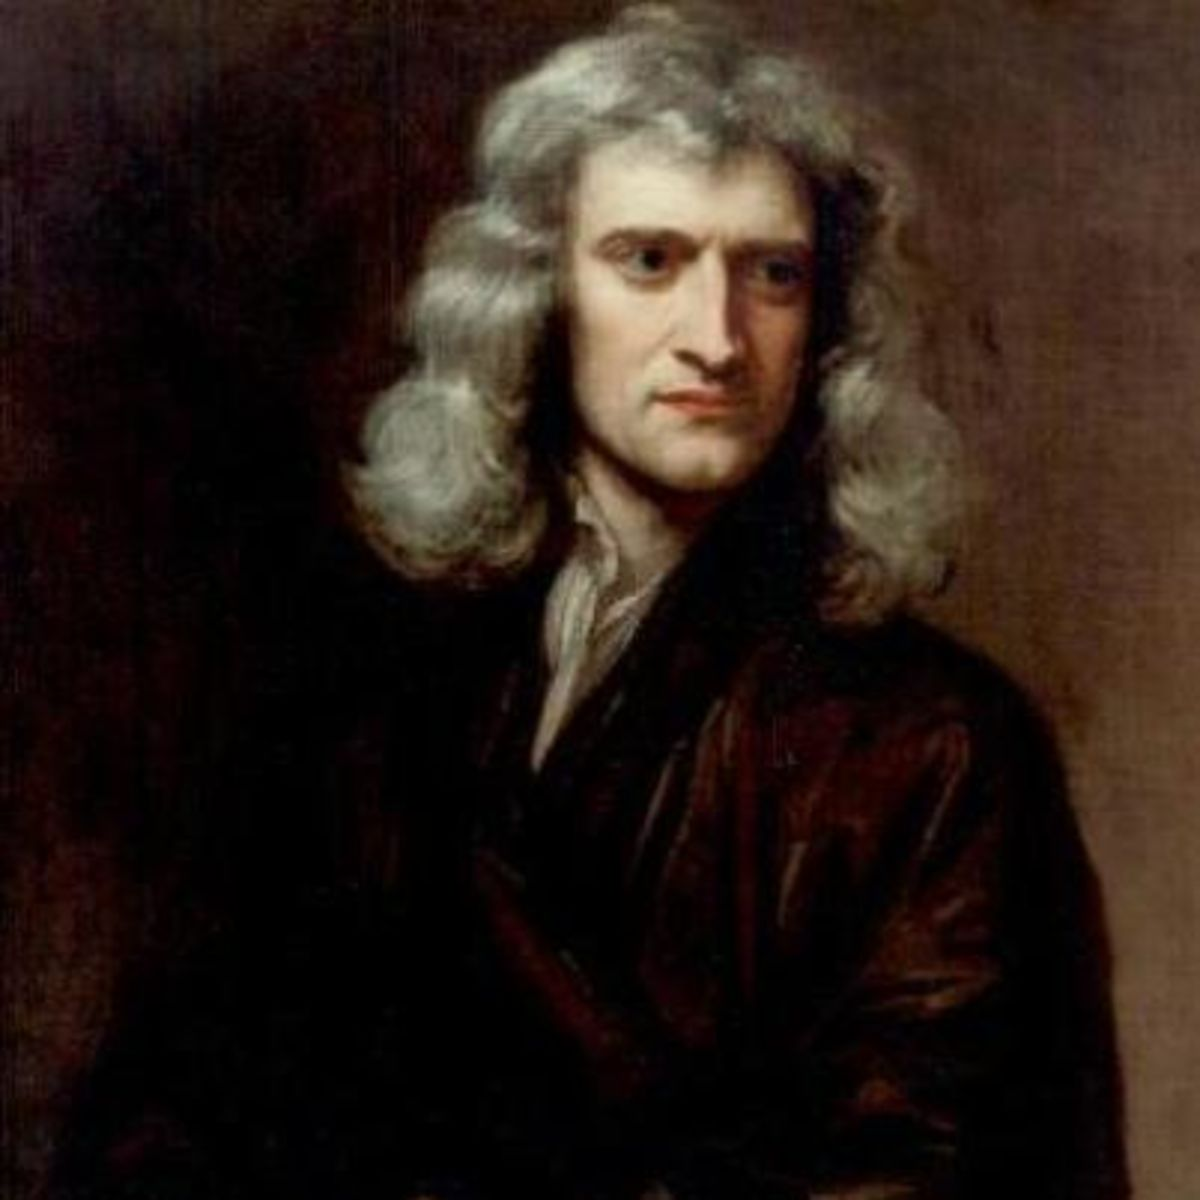
\includegraphics[height=.55\textheight]{images/newton}
		  		\end{center}
			\column{.6\textwidth}  		
				\begin{block}{Frase}
					\begin{center}
						{\large Eu consigo calcular \\o movimento dos corpos celestiais, \\mas não a loucura das pessoas.}
					\end{center}
				\end{block}		  		
		  		\begin{block}{Quem?}
		  			\begin{center}
						{\bf Isaac Newton (1643-1727)} \\ Físico inglês.
					\end{center}
				\end{block}
		\end{columns}
	\end{frame}
	
%------------------------------------------
	\section{Revisão}
	
\subsection{Medição}
	\begin{frame}{Medindo grandezas}
		\begin{block}{Descobrindo a física...}
			Medindo e comparando grandezas
		\end{block}
		\begin{block}{Grandezas}
			\begin{itemize}
				\item Comprimento, 
				\item Tempo, 
				\item Massa, 
				\item Temperatura, 
				\item Pressão, 
				\item Corrente elétrica...
			\end{itemize}
		\end{block}
	\end{frame}
	
	\begin{frame}{Medindo grandezas}
		\begin{block}{Como medimos uma grandeza}
			Comparando-a com um padrão
		\end{block}
		\begin{block}{Unidade}
			Medida de uma grandeza
		\end{block}
		\begin{block}{Exemplo}
			Metro é uma unidade de grandeza de comprimento
		\end{block}	
	\end{frame}
	
	\begin{frame}{Medindo grandezas}
		\begin{block}{Sistema Internacional de Unidades (SI)}
			\begin{itemize}
				\item 1971
				\item 14ª Conferência Geral de Pesos e Medidas
				\item Sete grandezas como fundamentais
			\end{itemize}
		\end{block}
		\begin{center}
			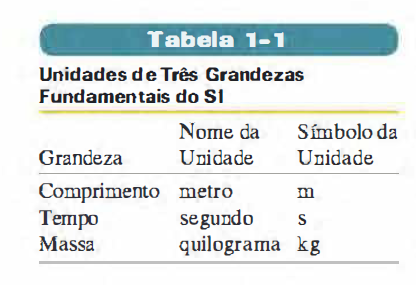
\includegraphics[scale=0.5]{images/tabela1-1.png}
		\end{center}
	\end{frame}
	
	\begin{frame}{Medindo grandezas}
		\begin{block}{Unidades Derivativas}
			São aquelas unidades que podem ser obtidas a partir de unidades fundamentais.
		\end{block}
		\begin{block}{Exemplo}
			1 watt = 1 W = 1 kg $\times m^2 / s^3$
		\end{block}
	\end{frame}
	
	\begin{frame}{Notação Científica}
		\begin{block}{Onde é utilizada?}
			Usa-se a notação científica para expressar as grandezas muito grandes.
		\end{block}
		\begin{block}{Formato}
			\begin{center}
				$a \times 10^b$
			\end{center}
			em que
			\begin{itemize}
				\item $a \in \mathbb{R}$ e $1 \leq a < 10$; e
				\item $b \in \mathbb{Z}^*$.
			\end{itemize}
		\end{block}
	\end{frame}
	
	\begin{frame}{Notação Científica}
		\begin{block}{Exemplos}
			\begin{itemize}
				\item 3.560.000.000 m = $3,56 \times 10^9$ m
				\item 0,000 000 492 s = $4,92 \times 10^{-7}$ s
			\end{itemize}
		\end{block}
		\begin{block}{Em linguagens de programação...}
			A notação abreviada normalmente é usada: \pause
			\begin{center}
				$7.59 e9$ ou $4.93 e-7$
			\end{center}
		\end{block}
		\begin{block}{Umas das utilidades...}
			Bastante útil no processo de conversão de unidades.
		\end{block}
	\end{frame}
	
	\begin{frame}{Uso de prefixos}
		\begin{center}
			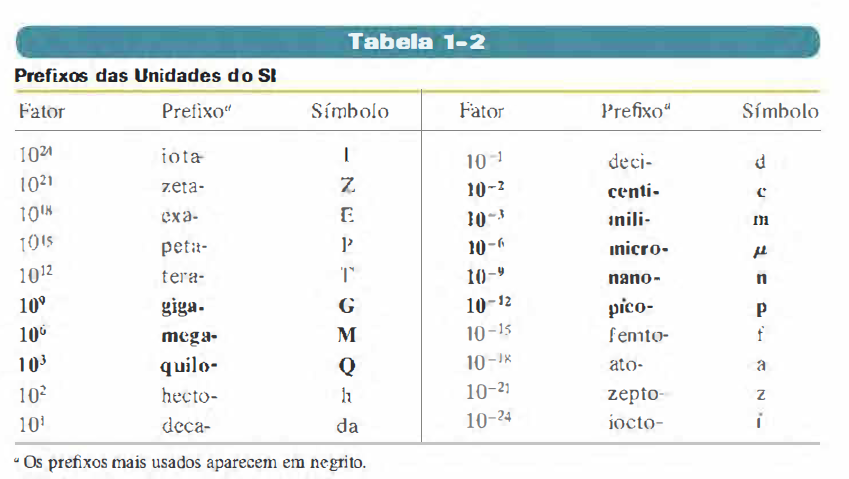
\includegraphics[scale=0.5]{images/tabela1-2.png}
		\end{center}
	\end{frame}
	
	\subsection{Comprimento}
	\begin{frame}{Medida de Comprimento}
		\begin{block}{Comprimento}
			No SI, a unidade para o comprimento é o metro (m).
		\end{block}
		\begin{block}{Metro}
			Distância percorrida pela luz no vácuo durante um intervalo de tempo de 1/299.792.458 de segundo.
		\end{block}
	\end{frame}
	
	\begin{frame}{Curiosidade}
		\begin{center}
			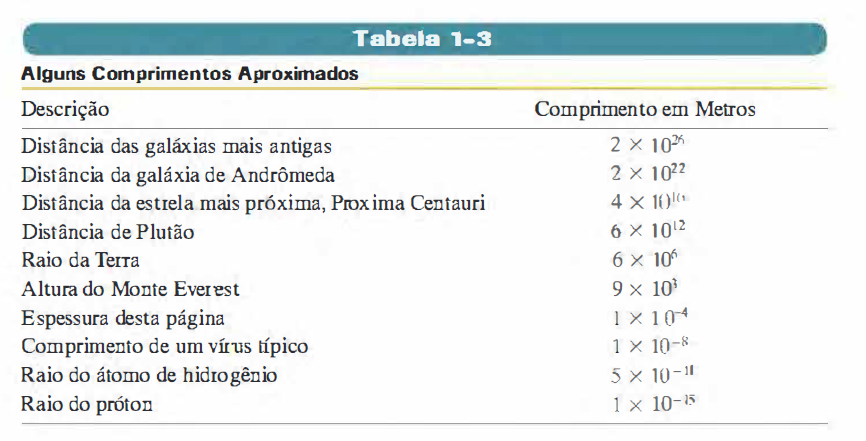
\includegraphics[scale=0.5]{images/tabela1-3.png}
		\end{center}
	\end{frame}
	
	\subsection{Tempo}
	\begin{frame}{Medida de Tempo}
		\begin{block}{Tempo}
			No SI, a unidade para o tempo é o segundo (s).
		\end{block}
		\begin{block}{Segundo}
			O intervalo de tempo que corresponde a 9.192.631.770 oscilações da luz (de um comprimento de onda especificado) emitida por um átomo de césio 133.
		\end{block}
		\begin{block}{Hora Coordenada Universal (UTC)}
			Fornecida por um relógio atômico no Colorado, EUA.
		\end{block}
	\end{frame}
	
	\begin{frame}{Curiosidade}
		\begin{center}
			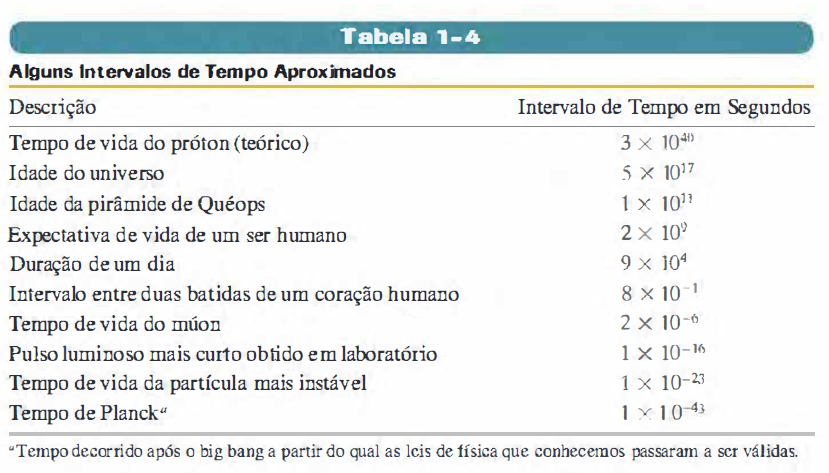
\includegraphics[scale=0.5]{images/tabela1-4.png}
		\end{center}
	\end{frame}
	
	\subsection{Massa}
	\begin{frame}{Medida de Massa}
		\begin{block}{Massa}
			No SI, a unidade para massa é o quilograma (kg).
		\end{block}
		\begin{block}{Quilograma}
			Um cilindro de platina irídio com 3,9cm de altura e 3,9cm de diâmetro.
		\end{block}
		\begin{center}
			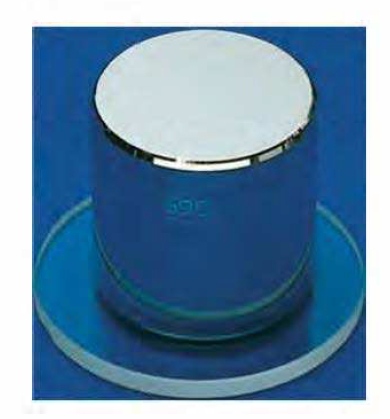
\includegraphics[scale=0.3]{images/figura1-3.png}
		\end{center}
	\end{frame}
	
	\begin{frame}{Curiosidade}
		\begin{center}
			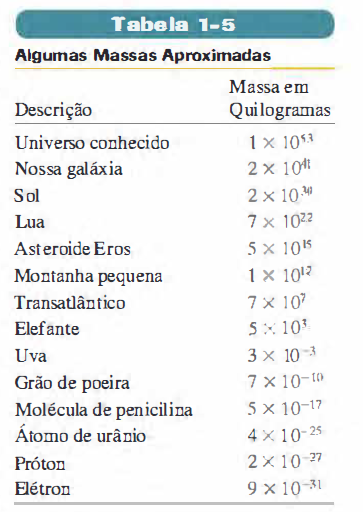
\includegraphics[scale=0.5]{images/tabela1-5.png}
		\end{center}
	\end{frame}	
	
	\begin{frame}{Massa Específica}
		\begin{block}{Massa específica}
			É a massa por unidade de volume.
			\begin{center}
				$\rho = \dfrac{m}{V}$
			\end{center}
		\end{block}
		\begin{block}{Exemplo: Massa específica da água}
			1 g/$\mbox{cm}^3$
		\end{block}
	\end{frame}

	\section{Movimento Retilíneo}
	\begin{frame}{O que é Física?}
		\begin{block}{Um dos objetivos da Física...}
			\begin{itemize}
				\item Estudar características do movimento; \pause
				\item Ex.: Rapidez com que eles se realizam.
			\end{itemize}
		\end{block} \pause
		\begin{block}{Aplicações}
			\begin{itemize}
				\item Engenheiros da NASCAR $\rightarrow$ desempenho de carros; \pause
				\item Médicos $\rightarrow$ mapeamento do fluxo de sangue; \pause
				\item Motoristas $\rightarrow$ redução de velocidade.
			\end{itemize}
		\end{block} \pause
		\begin{block}{Movimento Unidimensional}
			É o estudo do movimentos de objetos em linha reta.
		\end{block}
	\end{frame}

	\begin{frame}{Movimentos}
		\begin{block}{Movimento Unidimensional}
			Propriedade Gerais:
			\begin{itemize}
				\item Trajetória (retilínea): \pause
					\begin{itemize}
						\item vertical;
						\item horizontal; ou 
						\item inclinada.
					\end{itemize} \pause
				\item ``Forças'' que atuam sobre o objeto; \pause
					\begin{itemize}
						\item Velocidade;
						\item Direção..
					\end{itemize}
				\item Tipo de objeto:
					\begin{itemize}
						\item Partícula;
						\item Fluido...
					\end{itemize}
			\end{itemize}
		\end{block}
	\end{frame}

	\begin{frame}{Posição e Deslocamento}
		\begin{center}
			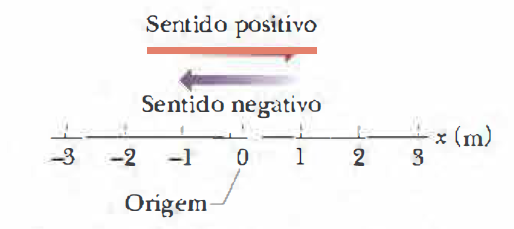
\includegraphics[scale=0.6]{images/fig2-1}
		\end{center}
		\begin{itemize}
			\item Ponto de referência: origem; \pause
			\item Sentido: positivo ou negativo; \pause
			\item Unidade de comprimento: m (por exemplo).
		\end{itemize}
	\end{frame}

	\begin{frame}{Posição e Deslocamento}
		\begin{block}{Deslocamento}
			A mudança de posição $x_1$ para a posição $x_2$ está associado a um {\bf deslocamento} $\Delta x$: \pause
			\begin{center}
				$\Delta x = x_2 - x_1$
			\end{center}
		\end{block} \pause
		\begin{block}{Símbolo $\Delta$}
			Associado à variação de grandezas, correspondendo à diferença entre os valores final e inicial.
		\end{block} \pause
		\begin{alertblock}{Cuidado!!!}
			Distância efetivamente percorrida é diferente de deslocamento.
		\end{alertblock}
	\end{frame}

	\begin{frame}{Posição e Deslocamento}
		\begin{block}{Deslocamento é uma grandeza vetorial}
			\begin{itemize} \pause
				\item Módulo; \pause
				\item Direção; \pause
				\item Sentido.
			\end{itemize}
		\end{block} \pause
		\begin{exampleblock}{Exercício}
			Considere três pares de posições iniciais e finais, respectivamente, ao longo do eixo x. A que pares correspondem deslocamentos negativos: 
				\begin{enumerate}
					\item -3 m, + 5 m; 
					\item -3 m, -7 m; 
					\item 7 m, -3 m.
				\end{enumerate}
		\end{exampleblock}
	\end{frame}

	\begin{frame}{Gráfico posição $\times$ tempo}
		\begin{center}
			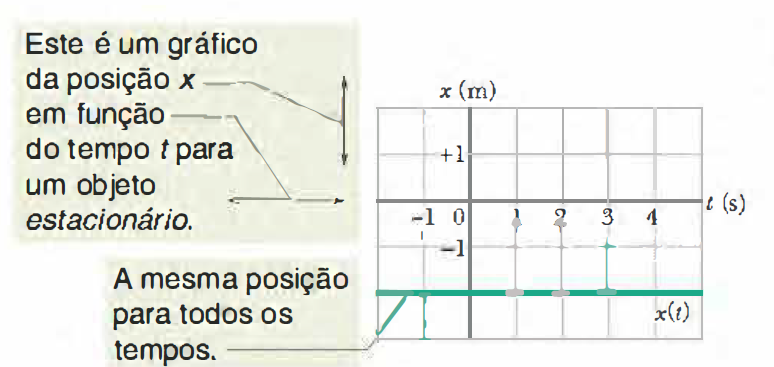
\includegraphics[scale=0.4]{images/fig2-2}
		\end{center}
		\begin{block}{Notação}
			$x(t)$ representa a função $x$ em relação a $t$.
		\end{block}
	\end{frame}

	\begin{frame}{Gráfico posição $\times$ tempo}
		\begin{center}
			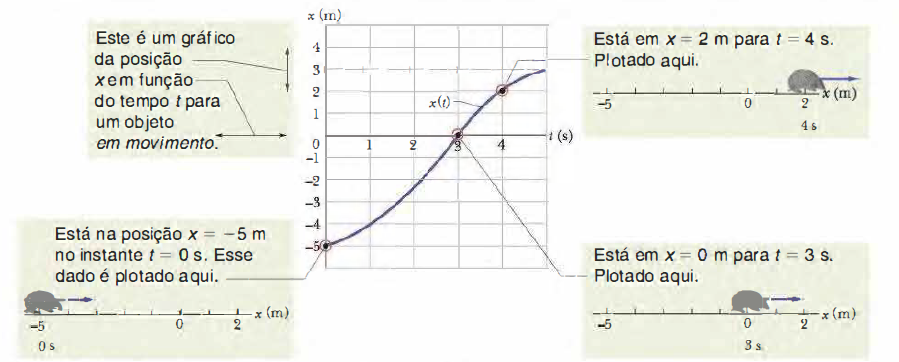
\includegraphics[scale=0.45]{images/fig2-3}
		\end{center}
	\end{frame}

	\begin{frame}{Velocidade Média}
		\begin{block}{Velocidade Média}
			\begin{center}
				v$_{\mbox{méd}} = \dfrac{\Delta x}{\Delta t} = \dfrac{x_2 - x_1}{t_2 - t_1}$
			\end{center} \pause
			\begin{itemize}
				\item $x_1$ é a posição no instante $t_1$; \pause
				\item $x_2$ é a posição no instante $t_2$; \pause
				\item No SI, a unidade de v$_{\mbox{méd}}$ é $m/s$; \pause
				\item v$_{\mbox{méd}}$ também é uma grandeza vetorial.
			\end{itemize}
		\end{block}
	\end{frame}

	\begin{frame}{Gráfico posição $\times$ tempo}
		\begin{center}
			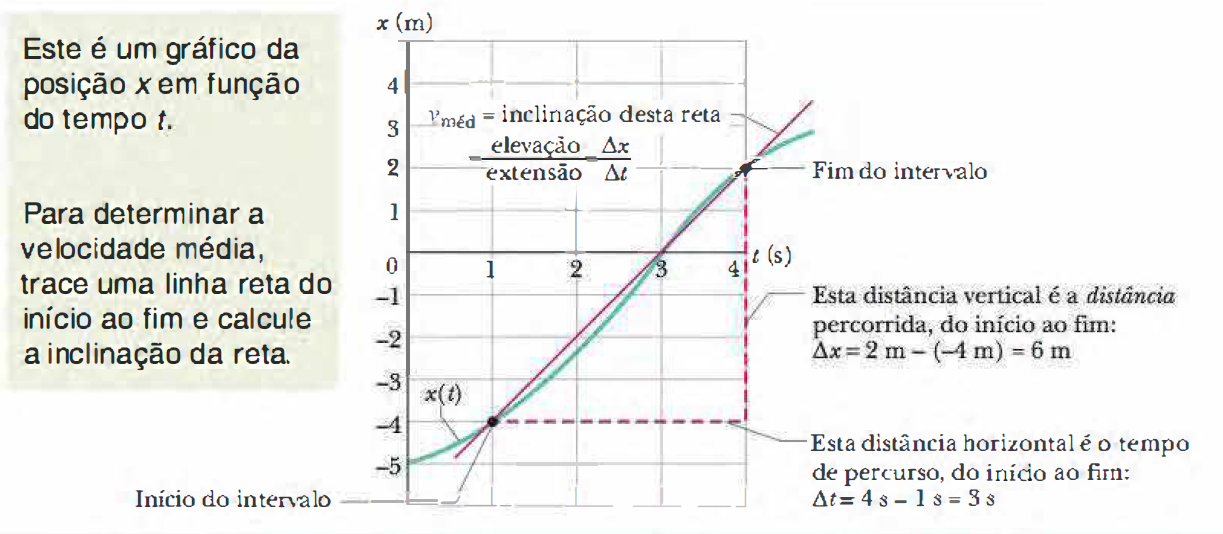
\includegraphics[scale=0.35]{images/fig2-4}
		\end{center}
	\end{frame}

	\begin{frame}{Velocidade Escalar Média}
		\begin{block}{Velocidade Escalar Média}
			\begin{center}
				s$_{\mbox{méd}} = \dfrac{\mbox{distância total}}{\Delta t} $
			\end{center} \pause
			\begin{itemize}
				\item s$_{\mbox{méd}}$ não é uma grandeza vetorial;
				\item o valor de s$_{\mbox{méd}}$ pode ser diferente do valor de v$_{\mbox{méd}}$.
			\end{itemize}
		\end{block}
	\end{frame}

	\begin{frame}{Velocidade Escalar Média}
		\begin{block}{Exercício}
			Depois de dirigir um carro em uma estrada retilínea por	8,4 km a 70 km/h, você para por falta de gasolina. Nos 30 min seguintes, você caminha por mais 2,0 km ao longo da estrada até chegar a um posto de gasolina.
				\begin{enumerate} \pause
					\item Qual foi o deslocamento total, do início da viagem até chegar ao posto de gasolina? \pause
					\item Qual é o intervalo de tempo $\Delta t$ entre o início da viagem e o instante em que você chega ao posto? 
				\end{enumerate}
			
		\end{block}
	\end{frame}

	\begin{frame}{Velocidade Escalar Média}
		\begin{block}{Exercício}
			Depois de dirigir um carro em uma estrada retilínea por	8,4 km a 70 km/h, você para por falta de gasolina. Nos 30 min seguintes, você caminha por mais 2,0 km ao longo da estrada até chegar a um posto de gasolina.
			\begin{enumerate} \pause
				\setcounter{enumi}{2}
				\item Qual é a velocidade média v$_{\mbox{méd}}$ do início da viagem até a chegada ao posto de gasolina? Determine a solução numericamente e graficamente. \pause
				\item Suponha que para encher um bujão de gasolina, pagar e caminhar de volta para o carro você leva 45 min. Qual é a velocidade escalar média do início da viagem até o momento em que você chega de volta ao lugar onde deixou o carro?
			\end{enumerate}
		\end{block}
	\end{frame}

	\begin{frame}{Gráfico posição $\times$ tempo}
		\begin{center}
			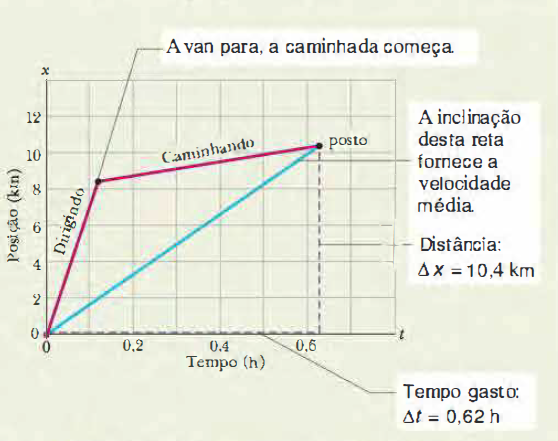
\includegraphics[scale=0.5]{images/fig2-5}
		\end{center}
	\end{frame}
	
	\begin{frame}{Bônus (0,5 pt)}
		\begin{block}{Desafio}
			{\bf (Halliday 3.23)} O oásis B está 25 m a leste do oásis A. Partindo do oásis A, um camelo percorre 24 m em uma direção $15^{\circ}$ ao sul do leste e 8,0 m para o norte. A que distância o camelo está do oásis B?
		\end{block} \pause
		\begin{block}{Informações úteis}
			\begin{itemize}
                \item Candidaturas (25 de outubro, 17h20);
                \item Resposta escrita e apresentação (27 de outubro, 19h00).
			\end{itemize}
		\end{block} 
	\end{frame}
	
	\begin{frame}
		\titlepage
	\end{frame}
	
\end{document}